\documentclass{sig-alternate}
%\documentclass{article}


\usepackage{enumitem}
\usepackage{framed}
\usepackage{cprotect}
\usepackage{enumitem}
\usepackage{listings}
\usepackage{amstext}
\usepackage{amstext}
\usepackage{pdfpages}
\usepackage{alltt}
\usepackage{epstopdf}
\usepackage{xspace,colortbl}
\usepackage[USenglish]{babel}
\usepackage{multirow}
\usepackage{url}
\usepackage{subfigure}
\usepackage{graphicx}%%
\usepackage{amssymb}
\usepackage{fmtcount}
\usepackage{amsfonts}
\usepackage{xspace}
\usepackage{amsmath}
\usepackage{multirow}
\usepackage[mathscr]{eucal}
%\usepackage{psfrag}
\usepackage{colortbl}

\usepackage{bm}
\usepackage{charter}
\usepackage[nospace]{cite}
\usepackage{csquotes}
\usepackage{enumitem}

\lstset{basicstyle=\large,breaklines=true,language=SQL,belowcaptionskip=.1\baselineskip}

%\linespread{0.975}

\makeatletter
\def\@copyrightspace{\relax}
\makeatother

\begin{document}

%\setlength{\belowdisplayskip}{1pt} \setlength{\belowdisplayshortskip}{1pt}
%\setlength{\abovedisplayskip}{1pt} \setlength{\abovedisplayshortskip}{1pt}
%\setlength{\belowcaptionskip}{-10pt}
%\selectfont

\newtheorem{theorem}{Theorem}
\newtheorem{example}{Example}
\newtheorem{definition}{Definition}
\newtheorem{problem}{Problem}
\newtheorem{property}{Property}
\newtheorem{proposition}{Proposition}
\newtheorem{lemma}{Lemma}
\newtheorem{corollary}{Corollary}

\newcommand{\cond}{\textrm{pred}\xspace}
\newcommand{\dataset}{data set\xspace}
\newcommand{\datasets}{data sets\xspace}
\newcommand{\spview}{\textsf{SPView}\xspace}
\newcommand{\fjview}{\textsf{FJView}\xspace}
\newcommand{\aggview}{\textsf{AggView}\xspace}
\newcommand{\hashfunc}[1]{\textsf{hash}(#1)\xspace}
\newcommand{\hashop}{\textsf{hash}\xspace}
\newcommand{\nsc}{\textsf{NormalizedSC}\xspace}
\newcommand{\rsc}{\textsf{RawSC}\xspace}

\newcommand{\avgfunc}{\ensuremath{\texttt{avg} }\xspace}
\newcommand{\maxfunc}{\ensuremath{\texttt{max} }\xspace}
\newcommand{\minfunc}{\ensuremath{\texttt{min} }\xspace}
\newcommand{\histfunc}{\ensuremath{\texttt{histogram\_numeric} }\xspace}
\newcommand{\countfunc}{\ensuremath{\texttt{count}}\xspace}
\newcommand{\sumfunc}{\ensuremath{\texttt{sum} }\xspace}
\newcommand{\varfunc}{\ensuremath{\texttt{var} }\xspace}
\newcommand{\stdfunc}{\ensuremath{\texttt{std} }\xspace}
\newcommand{\covfunc}{\ensuremath{\texttt{cov} }\xspace}
\newcommand{\corrfunc}{\ensuremath{\texttt{corr} }\xspace}
\newcommand{\medfunc}{\ensuremath{\texttt{median} }\xspace}
\newcommand{\percfunc}{\ensuremath{\texttt{percentile} }\xspace}
\newcommand{\havingfunc}{\ensuremath{\texttt{HAVING} }\xspace}
\newcommand{\selectfunc}{\ensuremath{\texttt{select} }\xspace}
\newcommand{\ratio}{\ensuremath{\rho }\xspace}


\newcommand{\insertion}{\ensuremath{\texttt{INSERT} }\xspace}
\newcommand{\update}{\ensuremath{\texttt{UPDATE} }\xspace}
\newcommand{\delete}{\ensuremath{\texttt{DELETE} }\xspace}

\newcommand{\sysfull}{ErrorPhobe\xspace}
\newcommand{\sys}{ErrorPhobe}
\newcommand{\sysM}{PC\xspace}
\newcommand{\sysnospace}{ActiveClean}

\newcommand{\tbl}[1]{\textsf{#1}\xspace}
\newcommand{\field}[1]{\textsf{#1}\xspace}
\newcommand{\cost}{\textrm{cost}\xspace}
\newcommand{\ans}{\textsf{ans}\xspace}
\newcommand{\dans}{\Delta\textsf{ans}\xspace}
\newcommand{\cqp}{correction query processing\xspace}
\newcommand{\Cqp}{Correction query processing\xspace}

\newcommand{\reminder}[1]{{{\textcolor{magenta}{\{\{\bf #1\}\}}}\xspace}}
\newcommand{\specialcell}[2][c]{%
  \begin{tabular}[#1]{@{}c@{}}#2\end{tabular}}

\def\ojoin{\setbox0=\hbox{$\bowtie$}%
  \rule[-.02ex]{.25em}{.4pt}\llap{\rule[\ht0]{.25em}{.4pt}}}
\def\leftouterjoin{\mathbin{\ojoin\mkern-5.8mu\bowtie}}
\def\rightouterjoin{\mathbin{\bowtie\mkern-5.8mu\ojoin}}
\def\fullouterjoin{\mathbin{\ojoin\mkern-5.8mu\bowtie\mkern-5.8mu\ojoin}}

%\setlength{\belowcaptionskip}{-10pt}

%\newcommand{\reminder}[1] {}
%\pagestyle{plain}

\title{A Library For Synthesizing Data Error}

%\numberofauthors{1}
%\author{\large Sanjay Krishnan, Jiannan Wang, Michael J. Franklin, Ken Goldberg, Tim Kraska{$\,^\dag$} \\
%\vspace{.2em}\affaddr{\large UC Berkeley, ~~ $^\dag$Brown University} \\
%\vspace{.1em}\affaddr{\large \{sanjaykrishnan, jnwang, franklin, goldberg\}@berkeley.edu}\\
%\affaddr{\large tim\_kraska@brown.edu}
%}

%\fontsize{10pt}{12pt}
%\selectfont

%\input{coverletter.tex}

\maketitle

\iffalse
\begin{abstract}
Data are susceptible to various forms of corruption such as missing, incorrect, or inconsistent values.
Almost all of the existing work in data cleaning assumes an interaction model where analysts have unrestricted access to the base data, which is not realistic in many situations concerning personal or sensitive information.
This paper explores a differential privacy mechanism that allows for downstream data cleaning and exploratory analysis.
We propose a framework called \sys which creates private views of a database using a generalization of the well-studied randomized response model.
For large enough datasets, we show thate errors are still detectable even in the private data and can be cleaned. 
We derive finite-sample bounds for estimates of aggregate queries on these cleaned private views.
Our analysis suggests that error is essentially linear in the privacy factor.
\end{abstract}
\fi


\section{Introduction}
Preparing and cleaning datasets prior to analysis is a perennial challenge in data analytics. As it has become easier to acquire and store ever larger datasets, the challenges associated with large-scale data cleaning, wherein issues caused by incorrect, missing, and duplicate data are identified and repaired, are of interest to both industry and academia. The result has been a several new systems, algorithms, abstractions, and interfaces for data cleaning --- however, there does not exist a unified evaluation methodology for either research or practice. This paper describes a number of problems in data cleaning and proposes new techniques to evaluate and benchmark data cleaning.


Important:

\begin{itemize}
\item Clearly distinguish training and testing and discuss how dirty data affects each of these settigns.
\item Important to mention that this is not comprehensive.  Lots of errors such as integration we DONT cover, or don't cover adequately.
\end{itemize}


\subsection{One Angle}

One source of challenges is that what dirtiness means, and how it should be resolved, is highly contextual.  It depends on the intended application---ML may not care about things close to the margin, stable aggregation functions such as median may be robust to noise---the complexity of the data (how normalized, how its modeled), etc etc.

Existing data cleaning systems take a scortched earth approach, where the entire dataset is cleaned.  In settings such as data integration, where the data will be individually presented to users (say in bills), this is needed.  However, many modern applications related to prediction and analysis do not need this approach. 

For exampel, give a simple example where understanding how robust the application is to data dirtiness is important.  Maybe the devolper/user can describe the types of dirtiness and wants to see how robust it will be.  

\subsection{Another Angle}

There are many many data cleaning algorithms that can be applied in different contexts, for different types of datasets, and at times for a specific type of data error.  (list types of data errors)   The current challenge is that it is unclear how they apply in a general application, and how they compare under other dirtiness settings, or when multiple data errors are present in a dataset.  This is a big limitation because it is currently difficult for practitioners to pick the most appropriate algorithms for their task.    On the bright side, [ref wisteria, etc] have proposed a small set of operators that can address a large variety of possible errors.  If we can understand when and how effectively each cleaning alogirthm is for a dataset and application, then we have hopes of realizing an optimizer for declarative data cleaning languages.  In this paper, we propose an extensible framework for making these evaluations, propose metrics, and show that a simple optimizer can be built.  In addition, we show other things that sanjay is excited about.


\begin{itemize}
    \item Describe the problems that we are addressing
    \item Describe the types of data errors
    \item Describe the types of cleaning software
    \item Describe the applications and potential utility to the world.
\end{itemize}


\section{Background}

\begin{itemize}
    \item Walk through an example ETL/Data Cleaning pipeline, how do you evaluate this, how do you test for issues, how do you test competing algorithms.
    \item Describe the current issues and challenges in evaluating data cleaning.
    \item Justify some of the key design decisions w.r.t language and tool for this specific project.
\end{itemize}

Despite all the different ways that data can be wrong, the they can be characterized by a concise set of declarative operations.  We base much of our approach for error synthesis and generation based on these operations.  LIST THEM.

Give examples for an operation that are seemingly different, but all boil down to the same operator.

Our insight is that the parameters to these operators are precisely what the domain experts can provide.

\subsection{Desirata}

Clarify how this relates to training and online prediction and where it benefits.  

1) Training a robust machine learning model.  Domain expert specifies the common sets of ways that the data can be dirty, and the system automatically, and increasingly perturbs the training dataset to understand how robust the trained model will be in the application.

2) The dual problem: online robustness.  Perturb the test dataset to see if the currently trained model is robust to future possible errors.

Generally characterizing dirtiness

3) Conversely, this simple algebra offers a concise way of {\it describing} the errors present in a dataset.  It is difficult to summarize data~\cite{bhardwaj2015collaborative}, and current approaches heavily utilize visualization or statistical summarization techniques, which can be difficult to understand.  In contrast, presenting a sequence of data error operations, along with their parameters, as a summary of a dirty dataset, would be akin to presenting a SQL query that summarizes a transformed dataset.  In fact, view synthesis work exists.



\subsection{Challenges}

{\bf Realistic errors:} recent studies have found that data cleaning algorithms that work on synthetic data can fail on real data errors~\cite{mikecleaningexp}.  However one of the main challenges is to 
collect, characterize, and use real-world data errors in a way that facilitates experimentation.  For instance, need both original dirty data as well as the cleaned versions, AND a mapping between the two datasets.
Once these are collected, these datasets are often used as-is.  However, an important property of benchmarks and robustness testers is the ability to scale up or down the amount of error in order to see how the data cleaning algorithms, and ultimately the application responds to the errors.  Without a model and characterization, difficult to even understand what this scaling means.

Thus, there is a fine balance between real examples and simulated errors.  A key challenges is to provide an extensible framework that grounds the types of errors using real datasets, but allows tunable parameters that allows for this scaling.

{\bf Characterization}  Given data, how to characterize?  Need to define operators, parameters, and generalizable methods to summarize the errors.  Much harder if there are multipel data errors present in the dataset.

{\bf Summarization: } ??




\section{Architecture}

This section describe the architecture of \sys.

\begin{figure}[ht]
  \centering
  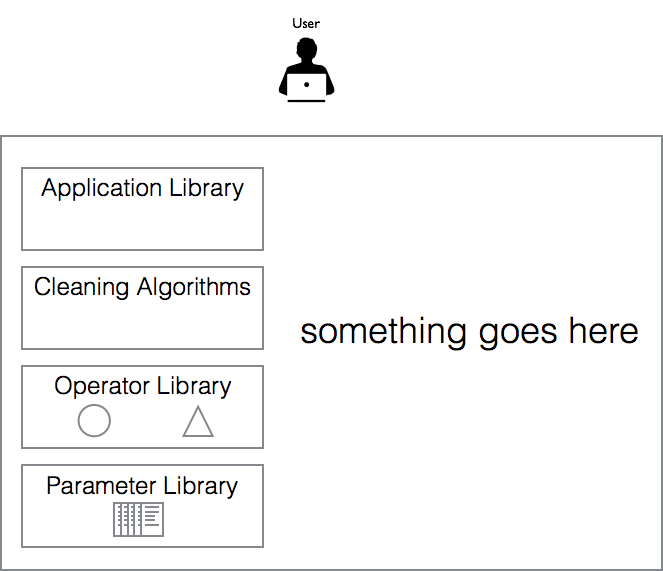
\includegraphics[width=.95\columnwidth]{figs/arch}
  \caption{}
  \label{f:arch}
\end{figure}


\begin{itemize}
    \item This section describes the architecture of the library
    \item Defines the api and all of the key components
    \item Forward references the research problems.
    \item Distinguish single function vs workflow.  The different problems it introduces: prov.
\end{itemize}


\subsection{A Model of Data Errors}


Logical error model: decomposing data erors into parameterized summaries/operations.  These form an error algebra.

Physical error model: The actual implementaitons.
\section{Dirty Data Models}

\begin{itemize}
    \item This section describes the process of generating the errors and cites places where such errors happen.
    \item Describe ER errors in more detail.
\end{itemize}
\section{Using the Synthesizer}

\subsection{Sensitivity Analysis}

\begin{itemize}
    \item This section describes how to evaluate the sensitivity of pipeline stages to error
\end{itemize}

\subsection{Summarizing Data Errors}

\begin{itemize}
    \item This subsection describes how we use the synthesizer to describe how a dataset is dirty.
\end{itemize}



\section{Experiments}
All of the experiments.
%\input{cleaning.tex}
%\input{queryprocessing.tex}
\section{Related Work}
There have also been a number of different proposals for both quantitative and qualitative data quality metrics~\cite{DBLP:journals/cacm/PipinoLW02, DBLP:journals/jdiq/CheahP15, DBLP:journals/jdiq/EvenS09,DBLP:journals/jdiq/SessionsV09, DBLP:journals/tkde/FanGLX11,DBLP:journals/sigmetrics/KeetonMW09}.
Most of the techniques rely on assessing the number of violated constraints or tests designed by the user, or qualitatively measure the number of erroneous decisions made by programs using the data.
In terms of probabilistic techniques, Sessions et al.~\cite{DBLP:journals/jdiq/SessionsV09} learn a Bayesian Network model to represent the data and measured how well the model fits the data.


Mention the data generator work  for synthesizing datasets with certain properites.   Also the subspace clustering benchmarks, maybe graph generators as well.


Backtesting and other robustness work.

Open AI Bench, UCI datastore.

%\input{conclusion.tex}

%\bibliographystyle{abbrv}
%\scriptsize
%\fontsize{8.4pt}{8.7pt} \selectfont
\bibliographystyle{abbrv}
\bibliography{ref} 
\clearpage
\normalsize \selectfont

\end{document}
